% Expt Fig 1: Loss curves L(t) are non-monotonic in the data-limited regime.
% Source figure: experiments/figures/01_overfit_demos/q2ext_individuals_overfit.pdf

\begin{figure}[t]
  \centering
  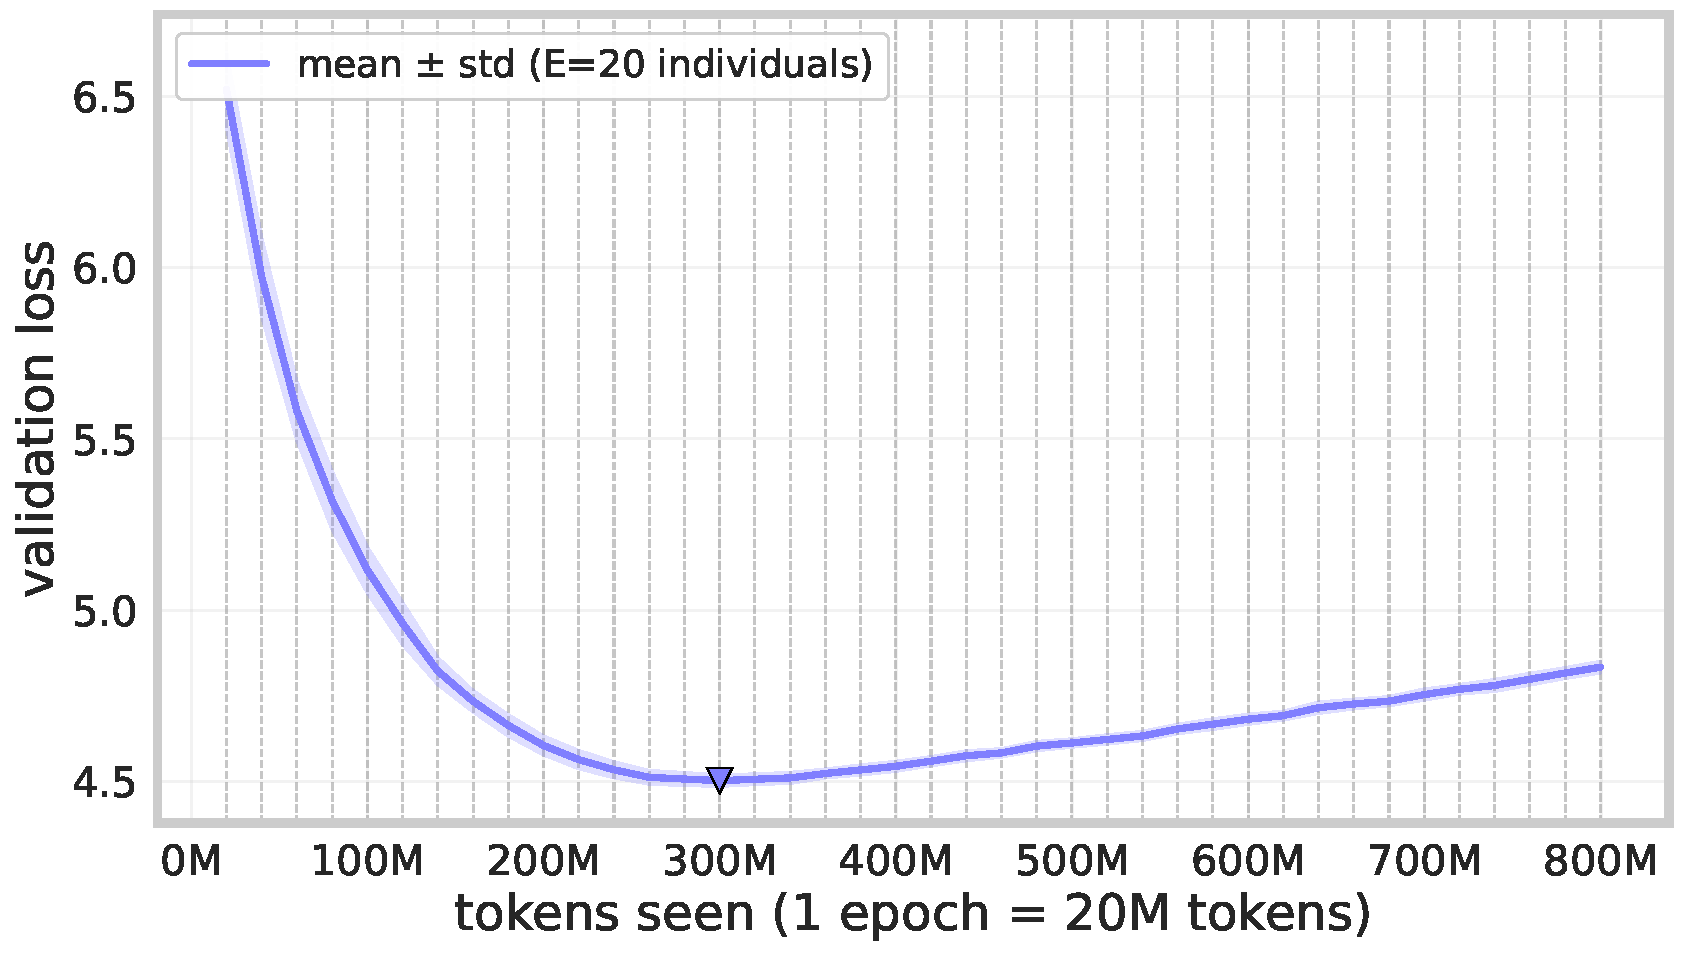
\includegraphics[width=0.85\linewidth]{experiments/figures/01_overfit_demos/q2ext_individuals_overfit.pdf}
  \caption{%
    Validation loss $L(t)$ is non-monotonic in the data-limited regime.
    Mean $\pm$ std across $E=20$ independently-initialized GPT models
    trained on a 20M-token FineWeb subset for 40 epochs.
  }
  \label{fig:overfit_u_curve}
\end{figure}


% --- Notes (figure detail; place near the figure or as a footnote) ---
% These are the experimental details that don't belong in the short caption.

\paragraph{Notes on Figure~\ref{fig:overfit_u_curve}.}
All 20 models are trained at $n_\text{layer}=12$, $n_\text{embd}=768$ on
a $df=0.2$ FineWeb subset, with constant learning rate and weight decay
$0.1$.
Vertical dashed lines mark each epoch boundary; their uniform spacing,
one line per 20M tokens, visualizes the unique-data size being repeated.
The mean curve descends to its minimum ($\blacktriangledown$) at roughly
300M tokens (epoch 15, i.e. fifteen full passes over the data), then
rises monotonically through the remainder of training and reaches
$4.83$ at 800M tokens, exceeding the minimum by $0.33$ nats.
The std at the minimum is $0.017$.


% --- Body paragraph (stresses non-monotonicity) ---

Single-pass extrapolations of compute-optimal training, such as Chinchilla
scaling, implicitly assume that $L(t)$ is a monotonically decreasing
function of training steps $t$: more training, lower loss.
In the data-limited regime, where the unique training set is small and
the model performs many passes over it, this assumption fails.
Figure~\ref{fig:overfit_u_curve} shows $L(t)$ for $E=20$ $d12\_w768$
GPT models on a 20M-token FineWeb subset.
Rather than continuing to descend, validation loss reaches a clear
minimum at roughly 300M cumulative tokens (epoch 15) and then increases
steadily for the remaining 25 epochs, ultimately exceeding the minimum
by $0.33$ nats.
The descent-then-ascent shape is highly reproducible across seeds
(std $\approx 0.02$ at the minimum), which establishes that
non-monotonicity is a structural feature of multi-epoch training in
the data-limited regime, not a stochastic artifact.
This observation motivates the rest of the paper: rather than chasing
further loss reduction by continued training on a fixed dataset, can we
reach a lower attainable loss by ensembling independently-trained
models, i.e. spending compute on $E$ rather than on $t$?
